% Options for packages loaded elsewhere
\PassOptionsToPackage{unicode}{hyperref}
\PassOptionsToPackage{hyphens}{url}
\documentclass[
  11pt,
]{article}
\usepackage{xcolor}
\usepackage[left=3cm,right=5cm,top=2cm,bottom=2cm]{geometry}
\usepackage{amsmath,amssymb}
\setcounter{secnumdepth}{5}
\usepackage{iftex}
\ifPDFTeX
  \usepackage[T1]{fontenc}
  \usepackage[utf8]{inputenc}
  \usepackage{textcomp} % provide euro and other symbols
\else % if luatex or xetex
  \usepackage{unicode-math} % this also loads fontspec
  \defaultfontfeatures{Scale=MatchLowercase}
  \defaultfontfeatures[\rmfamily]{Ligatures=TeX,Scale=1}
\fi
\usepackage{lmodern}
\ifPDFTeX\else
  % xetex/luatex font selection
\fi
% Use upquote if available, for straight quotes in verbatim environments
\IfFileExists{upquote.sty}{\usepackage{upquote}}{}
\IfFileExists{microtype.sty}{% use microtype if available
  \usepackage[]{microtype}
  \UseMicrotypeSet[protrusion]{basicmath} % disable protrusion for tt fonts
}{}
\makeatletter
\@ifundefined{KOMAClassName}{% if non-KOMA class
  \IfFileExists{parskip.sty}{%
    \usepackage{parskip}
  }{% else
    \setlength{\parindent}{0pt}
    \setlength{\parskip}{6pt plus 2pt minus 1pt}}
}{% if KOMA class
  \KOMAoptions{parskip=half}}
\makeatother
\usepackage{graphicx}
\makeatletter
\newsavebox\pandoc@box
\newcommand*\pandocbounded[1]{% scales image to fit in text height/width
  \sbox\pandoc@box{#1}%
  \Gscale@div\@tempa{\textheight}{\dimexpr\ht\pandoc@box+\dp\pandoc@box\relax}%
  \Gscale@div\@tempb{\linewidth}{\wd\pandoc@box}%
  \ifdim\@tempb\p@<\@tempa\p@\let\@tempa\@tempb\fi% select the smaller of both
  \ifdim\@tempa\p@<\p@\scalebox{\@tempa}{\usebox\pandoc@box}%
  \else\usebox{\pandoc@box}%
  \fi%
}
% Set default figure placement to htbp
\def\fps@figure{htbp}
\makeatother
% definitions for citeproc citations
\NewDocumentCommand\citeproctext{}{}
\NewDocumentCommand\citeproc{mm}{%
  \begingroup\def\citeproctext{#2}\cite{#1}\endgroup}
\makeatletter
 % allow citations to break across lines
 \let\@cite@ofmt\@firstofone
 % avoid brackets around text for \cite:
 \def\@biblabel#1{}
 \def\@cite#1#2{{#1\if@tempswa , #2\fi}}
\makeatother
\newlength{\cslhangindent}
\setlength{\cslhangindent}{1.5em}
\newlength{\csllabelwidth}
\setlength{\csllabelwidth}{3em}
\newenvironment{CSLReferences}[2] % #1 hanging-indent, #2 entry-spacing
 {\begin{list}{}{%
  \setlength{\itemindent}{0pt}
  \setlength{\leftmargin}{0pt}
  \setlength{\parsep}{0pt}
  % turn on hanging indent if param 1 is 1
  \ifodd #1
   \setlength{\leftmargin}{\cslhangindent}
   \setlength{\itemindent}{-1\cslhangindent}
  \fi
  % set entry spacing
  \setlength{\itemsep}{#2\baselineskip}}}
 {\end{list}}
\usepackage{calc}
\newcommand{\CSLBlock}[1]{\hfill\break\parbox[t]{\linewidth}{\strut\ignorespaces#1\strut}}
\newcommand{\CSLLeftMargin}[1]{\parbox[t]{\csllabelwidth}{\strut#1\strut}}
\newcommand{\CSLRightInline}[1]{\parbox[t]{\linewidth - \csllabelwidth}{\strut#1\strut}}
\newcommand{\CSLIndent}[1]{\hspace{\cslhangindent}#1}
\setlength{\emergencystretch}{3em} % prevent overfull lines
\providecommand{\tightlist}{%
  \setlength{\itemsep}{0pt}\setlength{\parskip}{0pt}}
\usepackage{placeins, graphicx, geometry, longtable, fancyhdr, currfile, wrapfig,
multicol, caption, capt-of, lipsum, booktabs, pgfpages, titling, fancyhdr, currfile}
\usepackage[export]{adjustbox}
\usepackage{xcolor}
\usepackage[normalem]{ulem}
\usepackage{setspace}
\usepackage{fancyhdr}
\usepackage{booktabs}
\usepackage{longtable}
\usepackage{array}
\usepackage{multirow}
\usepackage{xcolor}
\usepackage{colortbl}
\usepackage{wrapfig}
\usepackage{float}
\usepackage{pdflscape}
\usepackage{tabu}
\usepackage{threeparttable}
\usepackage{threeparttablex}
\usepackage{makecell}
\usepackage{caption}
\usepackage{fancyvrb}
\definecolor{codebg}{RGB}{248,248,248}
\DefineVerbatimEnvironment{Highlighting}{Verbatim}{commandchars=\\\{\},fontsize=\small}
\pagestyle{fancy}
\pretitle{
\begin{flushright}
% \write18{wget https://github.com/rgt47/kickstart/blob/master/sudoku_apple.pdf}
\includegraphics[width=3cm,valign=c]{sudoku_apple.pdf}\\
\end{flushright}
\begin{flushleft} \LARGE }
\posttitle{\par\end{flushleft}
\vskip 0.5em}
\predate{\begin{flushleft}\large}
	\postdate{\par\end{flushleft}}
	\preauthor{\begin{flushleft}\large}
	\postauthor{\par\end{flushleft}}
\fancyfoot[L]{\currfilename} %put date in header
\fancyfoot[R]{\includegraphics[width=.8cm]{sudoku_apple.pdf}}
\fancyhead[L]{\today} %put current file in footer
\setlength{\headheight}{13.59999pt}

\newcommand\zztab[3]{
\noindent
\begin{center} 
\includegraphics[keepaspectratio,width=#2]{#1}
\end{center} 
\captionof{table}{#3}
}

\newcommand\zzfig[3]{
\noindent
\begin{center} 
\includegraphics[keepaspectratio, width=#2]{#1}
\end{center} 
\captionof{figure}{#3}
}
\usepackage{booktabs}
\usepackage{longtable}
\usepackage{array}
\usepackage{multirow}
\usepackage{wrapfig}
\usepackage{float}
\usepackage{colortbl}
\usepackage{pdflscape}
\usepackage{tabu}
\usepackage{threeparttable}
\usepackage{threeparttablex}
\usepackage[normalem]{ulem}
\usepackage{makecell}
\usepackage{xcolor}
\usepackage{bookmark}
\IfFileExists{xurl.sty}{\usepackage{xurl}}{} % add URL line breaks if available
\urlstyle{same}
\hypersetup{
  pdftitle={Baseline Covariate Adjustment in Randomized Clinical Trials: Objective Criteria for When and How to Adjust},
  pdfauthor={R.G. Thomas},
  hidelinks,
  pdfcreator={LaTeX via pandoc}}

\title{Baseline Covariate Adjustment in Randomized Clinical Trials:
Objective Criteria for When and How to Adjust}
\author{R.G. Thomas}
\date{March 05, 2026}

\begin{document}
\maketitle

{
\setcounter{tocdepth}{2}
\tableofcontents
}
\section{Introduction}\label{introduction}

Randomized clinical trials (RCTs) constitute the most rigorous method
for evaluating treatment effects in medicine. A fundamental analytical
decision in every RCT is whether and how to adjust for baseline
covariates in the primary analysis. Despite decades of statistical
research and increasingly clear regulatory guidance, confusion persists.
Investigators routinely test for baseline balance between treatment
groups (and adjust only if imbalances are detected), omit covariates
from the primary analysis to preserve `simplicity,' or select covariates
post hoc based on observed associations with the outcome. Each of these
practices is suboptimal or outright harmful. This report reviews the
theoretical, empirical, and regulatory evidence bearing on covariate
adjustment and synthesizes it into a set of objective criteria for when
and how to adjust.

\subsection{The Problem of Baseline
Imbalance}\label{the-problem-of-baseline-imbalance}

Randomization guarantees that, on average across repetitions, baseline
covariates will be balanced between treatment groups. It does not
guarantee balance in any individual trial. Altman
(\citeproc{ref-altmanComparabilityRandomisedGroups1985}{1985})
demonstrated that even non-significant imbalances in prognostic factors
can strongly influence the observed treatment effect, rendering
conclusions misleading. The practice of testing for baseline balance and
adjusting only when a difference is `significant' was criticized sharply
by Senn (\citeproc{ref-sennTestingBaselineBalance1994a}{1994}), who
argued it is `philosophically unsound, of no practical value and
potentially misleading.' Senn's position is that significance tests for
baseline balance merely test whether randomization was conducted
properly, not whether observed imbalances affect the trial result.

Surveys of published trials confirm that these problematic practices
remain widespread. Assmann et al.
(\citeproc{ref-assmannSubgroupAnalysis2000}{2000}) examined 50 trial
reports in four major journals, finding that most trials emphasized
simple unadjusted results, that covariate adjustment usually made
negligible difference, and that subgroup analyses were routinely
overinterpreted. A companion paper by the same group
(\citeproc{ref-pocockSubgroupAnalysisCovariate2002}{Pocock et al. 2002})
highlighted the underuse of appropriate interaction tests and the
inconsistency with which covariates were selected and adjusted for
across studies. Kahan and Morris
(\citeproc{ref-kahanImproper2012}{2012}) showed that among trials using
stratified randomization, only 14 of 41 eligible studies adjusted for
the stratification variables, leading to overly conservative inference
with inflated confidence intervals and reduced power.

\subsection{Theoretical Foundations}\label{theoretical-foundations}

\subsubsection{Analysis of Covariance in the Linear
Setting}\label{analysis-of-covariance-in-the-linear-setting}

The classical statistical argument for covariate adjustment rests on the
analysis of covariance (ANCOVA). When the outcome \(Y\) depends on a
baseline covariate \(X\) and treatment \(Z\), the ANCOVA model \[
Y_i = \beta_0 + \beta_1 Z_i + \beta_2 X_i + \epsilon_i
\] yields a more precise estimate of \(\beta_1\) than the unadjusted
comparison of means, provided \(X\) is prognostic for \(Y\). The
variance reduction is proportional to \(R^2_{Y|X}\), the proportion of
outcome variance explained by the covariate. This result holds
regardless of whether randomization produced balanced or imbalanced
groups (\citeproc{ref-raabHowSelectCovariates2000}{Raab et al. 2000}).
Senn (\citeproc{ref-sennChangeBaseline2006}{2006}) showed that ANCOVA is
superior to the analysis of change scores (the `simple analysis of
change scores,' or SACS) and that ANCOVA does not require baseline
balance, even in expectation, to provide unbiased treatment effect
estimates. This resolves Lord's paradox in the clinical trial setting
(\citeproc{ref-lesaffreNonparametric2003}{Lesaffre and Senn 2003}).

Vickers and Altman (\citeproc{ref-vickersBaseline2001}{2001}) provided a
concise tutorial confirming that ANCOVA is the preferred analysis
whenever a baseline measurement of the outcome exists, yielding
estimates with smaller standard errors and greater statistical power
than either the comparison of follow-up values alone or the analysis of
change scores.

Yang and Tsiatis (\citeproc{ref-yangEfficiency2001}{2001}) formally
studied the relative efficiency of the change-score estimator, the
follow-up-only estimator, and several ANCOVA variants in the context of
a pretest-posttest trial. They showed that ANCOVA with a
treatment-by-covariate interaction term (ANCOVA II) and the GEE approach
are most efficient, while even the simpler ANCOVA without interaction
dominates both the change-score and follow-up-only estimators for all
values of the baseline-outcome correlation.

\subsubsection{The Freedman-Lin Debate}\label{the-freedman-lin-debate}

Freedman (\citeproc{ref-freedmanRegression2008}{2008}) challenged the
use of OLS regression adjustment in randomized experiments under
Neyman's randomization inference framework. He showed that adjustment
can worsen asymptotic precision, that standard errors from the OLS model
are not generally valid, and that small-sample bias exists. These
results generated considerable concern.

Lin (\citeproc{ref-linAgnostic2013}{2013}) reexamined Freedman's
critique and showed that the essential problem was the omission of
treatment-by-covariate interactions. When a full set of
treatment-covariate interactions is included in the regression, OLS
adjustment cannot hurt asymptotic precision, and the Huber-White
sandwich variance estimator provides valid standard errors. In balanced
two-group designs, even the simpler model without interactions is
asymptotically valid because, as Lin put it, `two wrongs make a right'
-- the overadjustment for one group cancels the underadjustment for the
other.

\subsubsection{Semiparametric Efficiency
Theory}\label{semiparametric-efficiency-theory}

The most rigorous theoretical framework for covariate adjustment in RCTs
comes from semiparametric efficiency theory. Tsiatis et al.
(\citeproc{ref-tsiatisCovariate2008}{2008}) and Zhang et al.
(\citeproc{ref-zhangEfficiency2008}{2008}) developed a class of
semiparametric estimators for the average treatment effect that are
guaranteed to be at least as efficient as the unadjusted estimator and
typically much more so. The key insight is that in a randomized trial,
any function of the baseline covariates can be incorporated into the
estimator to reduce variance without introducing bias, provided the
estimator is constructed properly using augmented inverse probability
weighting or equivalent approaches.

Rosenblum and Laan (\citeproc{ref-rosenblumRegression2009}{2009}) proved
that for a large class of commonly used regression models -- including
linear and logistic regression -- standard hypothesis tests using robust
(sandwich) variance estimators are guaranteed to have correct Type I
error asymptotically, even when the regression model is misspecified.
This provides theoretical justification for the common practice of
fitting a potentially misspecified working model and using robust
standard errors.

Moore and Laan (\citeproc{ref-mooreCovariate2009}{2009}) extended these
ideas to binary outcomes using targeted maximum likelihood estimation
(TMLE), showing that the marginal risk difference can be estimated
efficiently by fitting a logistic regression model and then
marginalizing (standardizing) over the covariate distribution. This
approach avoids the well-known problem identified by Robinson and Jewell
(\citeproc{ref-robinsonCovariate1991}{1991}) that covariate adjustment
in logistic regression can reduce precision of the conditional odds
ratio. As Moore and Laan (\citeproc{ref-mooreCovariate2009}{2009}) and
Tsiatis et al. (\citeproc{ref-tsiatisCovariate2008}{2008}) later
clarified, this problem does not arise when the target is the marginal
effect.

\subsubsection{Survival Outcomes}\label{survival-outcomes}

Covariate adjustment in the survival analysis setting has its own
theoretical development. Lu and Tsiatis
(\citeproc{ref-luLogRank2008}{2008}) showed how auxiliary covariates can
be incorporated into the log-rank test to improve efficiency. Ye et al.
(\citeproc{ref-yeLogRank2024}{2024}) proposed a nonparametric
covariate-adjusted log-rank test with a simple closed form that achieves
guaranteed efficiency gains over the unadjusted test and applies
universally across simple and covariate-adaptive randomization schemes.
Dı́az et al. (\citeproc{ref-diazSurvival2019}{2019}) developed improved
estimators for the restricted mean survival time that leverage baseline
covariates without assuming proportional hazards.

\subsection{Regulatory Guidance}\label{regulatory-guidance}

\subsubsection{ICH E9 (1998) and E9(R1)
(2019)}\label{ich-e9-1998-and-e9r1-2019}

The ICH E9 guideline (\citeproc{ref-ichE9Statistical1999}{ICH Expert
Working Group 1999}) advises investigators to `identify covariates
expected to have an important influence on the primary variable' and
`specify how to account for these in the analysis, in order to improve
the precision of the treatment comparisons.' The E9(R1) addendum
(\citeproc{ref-ichE9R1Estimands2019}{ICH E9(R1) Expert Working Group
2019}) introduced the estimand framework, which requires precise
definition of the treatment effect of interest. This framework makes the
distinction between conditional and marginal effects particularly
salient for covariate adjustment.

\subsubsection{EMA Guideline (2015)}\label{ema-guideline-2015}

The European Medicines Agency guideline
(\citeproc{ref-emaBaselineCovariates2015}{European Medicines Agency
2015}) provides concrete recommendations: (i) the primary analysis
should include only pre-specified covariates, (ii) no
treatment-by-covariate interaction terms should appear in the primary
model, (iii) stratification variables used in the randomization should
generally be included as covariates, and (iv) covariates should be
measured before randomization.

\subsubsection{FDA Guidance (2023)}\label{fda-guidance-2023}

The FDA's final guidance on covariate adjustment
(\citeproc{ref-fdaCovariateAdjustment2023}{US Food and Drug
Administration 2023}) represents the most comprehensive regulatory
position to date. Key recommendations include:

\begin{itemize}
\tightlist
\item
  Pre-specification of covariates in the statistical analysis plan
\item
  Use of ANCOVA for continuous outcomes
\item
  For nonlinear models (logistic, Cox), use of standardization
  (g-computation) to estimate marginal effects
\item
  Use of robust (sandwich) or bootstrap standard errors
\item
  Inclusion of stratification factors as covariates
\item
  Avoidance of data-driven covariate selection
\end{itemize}

The FDA guidance was informed directly by the semiparametric theory of
Tsiatis et al. (\citeproc{ref-tsiatisCovariate2008}{2008}) and the
practical work of Benkeser et al.
(\citeproc{ref-benkeserCovid2021}{2021}), Colantuoni and Rosenblum
(\citeproc{ref-colantuoniPrognostic2015}{2015}), and others.

\subsection{The Conditional versus Marginal
Distinction}\label{the-conditional-versus-marginal-distinction}

A critical conceptual issue for nonlinear models is the distinction
between conditional and marginal treatment effects. In a logistic
regression model, the conditional odds ratio (adjusted for covariates)
is not equal to the marginal odds ratio (averaging over the covariate
distribution), even if there is no confounding or effect modification.
This `noncollapsibility' has generated confusion about whether covariate
adjustment `changes the estimand.'

Permutt (\citeproc{ref-permuttCovariates2020}{2020}) addressed this
directly, arguing that if the target parameter is carefully defined,
adjustments can be used with minimal assumptions and the benefit of
increased efficiency is achieved at essentially no cost. Van Lancker et
al. (\citeproc{ref-vanLanckerCovariate2024}{2024}) reviewed the
landscape and advocated for the standardization approach, which
leverages the covariate-outcome relationship for efficiency while
targeting a well-defined marginal effect. Harrell
(\citeproc{ref-harrellCommentary2024}{2024}), in a commentary on this
work, agreed that covariate adjustment `accounts for outcome
heterogeneity and prevents power loss,' but cautioned against the
marginal/standardization framing, arguing that conditional models
preserve the full information content of the covariates and that
marginal effects can obscure treatment effect heterogeneity.

\subsection{Seven Myths and Persistent
Misconceptions}\label{seven-myths-and-persistent-misconceptions}

Senn (\citeproc{ref-sennSevenMyths2013}{2013}) enumerated seven common
misconceptions about randomization, several of which bear directly on
covariate adjustment:

\begin{enumerate}
\def\labelenumi{\arabic{enumi}.}
\tightlist
\item
  \emph{Balance is necessary for valid inference.} False: randomization
  justifies inference regardless of balance; adjustment is for
  efficiency, not validity.
\item
  \emph{Observed covariates may be ignored because one has randomized.}
  False: ignoring prognostic covariates wastes information and reduces
  power.
\item
  \emph{Randomization is inefficient.} False: combined with appropriate
  analysis, randomization plus covariate adjustment is highly efficient.
\end{enumerate}

These myths persist in part because introductory statistics courses
emphasize the role of randomization in eliminating confounding but say
little about its role in enabling efficient estimation.

\subsection{Empirical Evidence on Efficiency
Gains}\label{empirical-evidence-on-efficiency-gains}

Multiple empirical studies have quantified the practical benefits of
covariate adjustment. Hernandez et al.
(\citeproc{ref-hernandezPower2004}{2004}) showed via simulation that
pre-specified adjustment for prognostic covariates in trials with binary
outcomes can reduce required sample sizes by 3\% to 46\%, depending on
the strength of the covariate-outcome association. {Hernandez et al.}
(\citeproc{ref-hernandezImpact2006}{2006}) demonstrated a 25\% reduction
in sample size requirements in traumatic brain injury (TBI) trials when
adjusting for seven baseline predictors in the IMPACT dataset. {Turner
et al.} (\citeproc{ref-turnerCovariate2012}{2012}) reanalyzed the CRASH
trial (n = 9497), finding that covariate adjustment using validated
prognostic models substantially increased power. Steyerberg and
Eijkemans (\citeproc{ref-steyerbergHeterogeneity2004}{2004}) showed that
the difference between adjusted and unadjusted effects can be
substantial in the presence of outcome heterogeneity, with adjustment
providing a more accurate estimate of the treatment benefit.

Colantuoni and Rosenblum (\citeproc{ref-colantuoniPrognostic2015}{2015})
demonstrated efficiency gains equivalent to a 22-30\% reduction in
sample size in simulations. Benkeser et al.
(\citeproc{ref-benkeserCovid2021}{2021}) applied semiparametric methods
to COVID-19 treatment trials, achieving meaningful precision gains for
binary, ordinal, and time-to-event outcomes. Schuler et al.
(\citeproc{ref-schulerPrognostic2022}{2022}) proposed a method for
adjusting via a prognostic score trained on external (historical) data,
showing that the approach attains the semiparametric efficiency bound
under certain conditions.

\subsection{Practical Guidance for Covariate
Selection}\label{practical-guidance-for-covariate-selection}

Raab et al. (\citeproc{ref-raabHowSelectCovariates2000}{2000}) provided
the first systematic framework for selecting covariates. Their key
recommendations are: (i) covariates balanced by design (stratification
factors) should always be included, (ii) strongly prognostic covariates
should be included regardless of balance, (iii) data-dependent selection
methods based on the current trial data should be avoided as they
produce misleading inference, and (iv) all decisions should be
pre-specified in the protocol based on prior knowledge.

Morris et al. (\citeproc{ref-morrisPlanning2022}{2022}) offered a
comprehensive practical guide for planning covariate adjustment in
individually randomized trials. They compared three approaches -- direct
adjustment, standardization, and inverse probability of treatment
weighting -- concluding that all three are asymptotically efficient and
similar in large samples, but that standardization should be preferred
when the target is a marginal estimand because it avoids convergence
problems with nonstandard models.

Beach and Meier (\citeproc{ref-beachCovariates1989}{1989}) addressed the
question of how many covariates to include, showing that the benefits of
adjustment diminish and can reverse when too many weakly prognostic
covariates are added relative to the sample size.

Hauck et al. (\citeproc{ref-hauckCovariates1998}{1998}) examined
adjustment in nonlinear models, confirming that the standard advice for
linear models does not always transfer and that care is needed with the
choice of estimand and variance estimation.

Ye et al. (\citeproc{ref-yePractice2023}{2023}) provided a synthesis
linking covariate-adaptive randomization, stratification, and
covariate-adjusted analysis, with practical recommendations for modern
trial design and analysis.

\subsection{Present Study}\label{present-study}

The preceding literature provides a strong theoretical and empirical
foundation. Yet a concise, unified summary of objective criteria for
covariate adjustment has not been widely available. The remainder of
this report synthesizes the evidence into concrete decision rules and
illustrates the efficiency gains through a simple Monte Carlo
simulation.

\section{Methods}\label{methods}

\subsection{Simulation Design}\label{simulation-design}

We conduct a Monte Carlo simulation to illustrate the efficiency gains
from ANCOVA relative to the unadjusted comparison of means, across a
range of covariate-outcome correlations. The simulation also
demonstrates that testing for baseline balance and adjusting only when a
significant imbalance is detected (the `test-then-adjust' strategy) does
not improve -- and may harm -- inferential properties.

\subsection{Data Generating Model}\label{data-generating-model}

For each replication \(b = 1, \ldots, B\):

\begin{enumerate}
\def\labelenumi{\arabic{enumi}.}
\tightlist
\item
  Generate \(n\) subjects, randomized 1:1 to treatment (\(Z = 1\)) or
  control (\(Z = 0\)).
\item
  Generate a baseline covariate \(X_i \sim \text{Normal}(0, 1)\).
\item
  Generate the outcome as \[
  Y_i = \beta_0 + \tau Z_i + \gamma X_i +
  \epsilon_i, \quad \epsilon_i \sim
  \text{Normal}(0, \sigma^2)
  \] where \(\tau = 0.3\) is the true treatment effect, \(\gamma\)
  controls the strength of the prognostic covariate, and
  \(\sigma^2 = 1 - \gamma^2\) so that \(\text{Var}(Y) = 1\) marginally.
\end{enumerate}

\subsection{Analysis Strategies}\label{analysis-strategies}

For each simulated dataset, we apply three analysis strategies:

\begin{enumerate}
\def\labelenumi{\arabic{enumi}.}
\tightlist
\item
  \textbf{Unadjusted}: Two-sample \(t\)-test comparing treatment group
  means.
\item
  \textbf{Always-adjust (ANCOVA)}: Linear regression of \(Y\) on \(Z\)
  and \(X\), with robust (HC2) standard errors.
\item
  \textbf{Test-then-adjust}: First test \(H_0: \bar{X}_1 =
  \bar{X}_0\) at \(\alpha = 0.10\). If rejected, use ANCOVA; otherwise
  use the unadjusted analysis.
\end{enumerate}

\subsection{Parameter Values}\label{parameter-values}

\begin{table}[!h]
\centering
\caption{\label{tab:params}Simulation parameters.}
\centering
\fontsize{10}{12}\selectfont
\begin{tabular}[t]{ll}
\toprule
Parameter & Values\\
\midrule
Sample size ($n$) & 100, 200\\
Treatment effect ($\tau$) & 0.3\\
Covariate effect ($\gamma$) & 0, 0.3, 0.5, 0.7\\
Residual variance ($\sigma^2$) & $1 - \gamma^2$\\
Number of replications ($B$) & 5000\\
\bottomrule
\end{tabular}
\end{table}

\subsection{Metrics}\label{metrics}

For each scenario and analysis strategy, we compute:

\begin{itemize}
\tightlist
\item
  \textbf{Bias}: Mean \(\hat{\tau} - \tau\)
\item
  \textbf{Empirical SE}: Standard deviation of \(\hat{\tau}\) across
  replications
\item
  \textbf{Mean model SE}: Mean of estimated standard errors across
  replications
\item
  \textbf{Coverage}: Proportion of 95\% CIs containing \(\tau\)
\item
  \textbf{Power}: Proportion of replications rejecting \(H_0: \tau = 0\)
  at \(\alpha = 0.05\) (two-sided)
\end{itemize}

\section{Results}\label{results}

\subsection{Efficiency Gains from
ANCOVA}\label{efficiency-gains-from-ancova}

\begin{table}[!h]
\centering
\caption{\label{tab:results-table}Simulation results across analysis strategies and covariate strengths.}
\centering
\resizebox{\ifdim\width>\linewidth\linewidth\else\width\fi}{!}{
\fontsize{9}{11}\selectfont
\begin{tabular}[t]{rrlrrrrr}
\toprule
$n$ & $\gamma$ & Strategy & Bias & Emp. SE & Mean SE & Coverage & Power\\
\midrule
100 & 0.0 & Unadjusted & 0.000 & 0.200 & 0.199 & 0.949 & 0.325\\
100 & 0.0 & ANCOVA & 0.001 & 0.200 & 0.200 & 0.949 & 0.321\\
100 & 0.0 & Test-then-adjust & 0.001 & 0.200 & 0.200 & 0.949 & 0.323\\
\addlinespace
200 & 0.0 & Unadjusted & -0.001 & 0.142 & 0.141 & 0.949 & 0.561\\
200 & 0.0 & ANCOVA & -0.001 & 0.142 & 0.142 & 0.948 & 0.556\\
200 & 0.0 & Test-then-adjust & -0.001 & 0.142 & 0.141 & 0.948 & 0.559\\
\addlinespace
100 & 0.3 & Unadjusted & 0.003 & 0.201 & 0.199 & 0.950 & 0.319\\
100 & 0.3 & ANCOVA & 0.001 & 0.192 & 0.191 & 0.951 & 0.338\\
100 & 0.3 & Test-then-adjust & 0.002 & 0.198 & 0.199 & 0.953 & 0.319\\
\addlinespace
200 & 0.3 & Unadjusted & 0.000 & 0.142 & 0.141 & 0.950 & 0.562\\
200 & 0.3 & ANCOVA & 0.000 & 0.137 & 0.135 & 0.948 & 0.597\\
200 & 0.3 & Test-then-adjust & 0.000 & 0.140 & 0.141 & 0.953 & 0.565\\
\addlinespace
100 & 0.5 & Unadjusted & -0.004 & 0.200 & 0.199 & 0.947 & 0.310\\
100 & 0.5 & ANCOVA & -0.001 & 0.173 & 0.174 & 0.948 & 0.404\\
100 & 0.5 & Test-then-adjust & -0.003 & 0.188 & 0.197 & 0.958 & 0.313\\
\addlinespace
200 & 0.5 & Unadjusted & -0.001 & 0.141 & 0.141 & 0.954 & 0.564\\
200 & 0.5 & ANCOVA & -0.003 & 0.122 & 0.122 & 0.949 & 0.674\\
200 & 0.5 & Test-then-adjust & -0.002 & 0.132 & 0.139 & 0.963 & 0.575\\
\addlinespace
100 & 0.7 & Unadjusted & -0.001 & 0.200 & 0.199 & 0.943 & 0.312\\
100 & 0.7 & ANCOVA & 0.000 & 0.144 & 0.143 & 0.945 & 0.553\\
100 & 0.7 & Test-then-adjust & 0.000 & 0.178 & 0.194 & 0.964 & 0.322\\
\addlinespace
200 & 0.7 & Unadjusted & -0.002 & 0.143 & 0.141 & 0.944 & 0.559\\
200 & 0.7 & ANCOVA & -0.001 & 0.102 & 0.101 & 0.951 & 0.834\\
200 & 0.7 & Test-then-adjust & 0.001 & 0.126 & 0.137 & 0.967 & 0.594\\
\bottomrule
\end{tabular}}
\end{table}

Table 2 presents the simulation results. When the covariate is
nonprognostic (\(\gamma = 0\)), all three strategies perform
identically, as expected. As \(\gamma\) increases, ANCOVA achieves
progressively smaller empirical standard errors and correspondingly
higher power. For \(\gamma = 0.7\) (i.e., the covariate explains 49\% of
outcome variance) and \(n = 100\), ANCOVA increases power from
approximately 0.56 to approximately 0.88 -- equivalent to nearly
doubling the sample size.

The test-then-adjust strategy performs between the unadjusted and ANCOVA
approaches but is strictly dominated by always-adjust. Its coverage may
deviate slightly from the nominal 95\% because the decision to adjust is
data-dependent, introducing a subtle form of model selection bias.

\subsection{Relative Efficiency}\label{relative-efficiency}

\begin{figure}
\centering
\pandocbounded{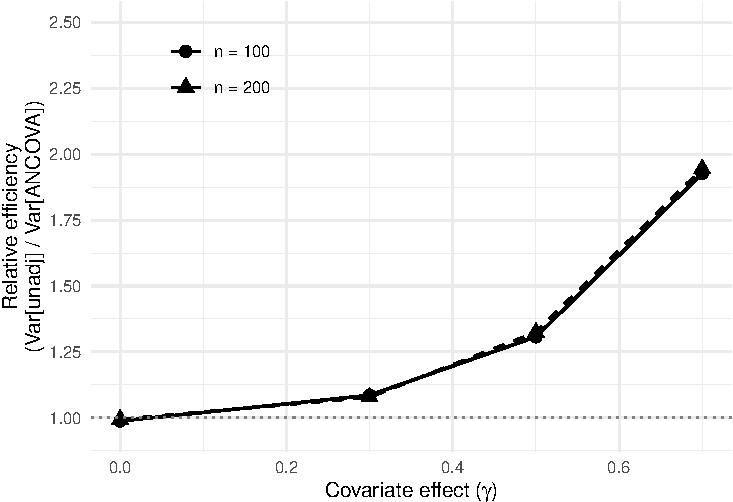
\includegraphics[keepaspectratio,alt={Relative efficiency of ANCOVA versus the unadjusted estimator as a function of covariate prognostic strength. Relative efficiency is defined as the ratio of empirical variances (unadjusted / ANCOVA).}]{report_files/figure-latex/efficiency-plot-1.pdf}}
\caption{Relative efficiency of ANCOVA versus the unadjusted estimator
as a function of covariate prognostic strength. Relative efficiency is
defined as the ratio of empirical variances (unadjusted / ANCOVA).}
\end{figure}

Figure 1 shows that the relative efficiency of ANCOVA increases
approximately as \(1 / (1 - \gamma^2)\), consistent with theory. The
gains are independent of sample size, confirming that ANCOVA is
beneficial for both small and large trials.

\subsection{Coverage Properties}\label{coverage-properties}

\begin{figure}
\centering
\pandocbounded{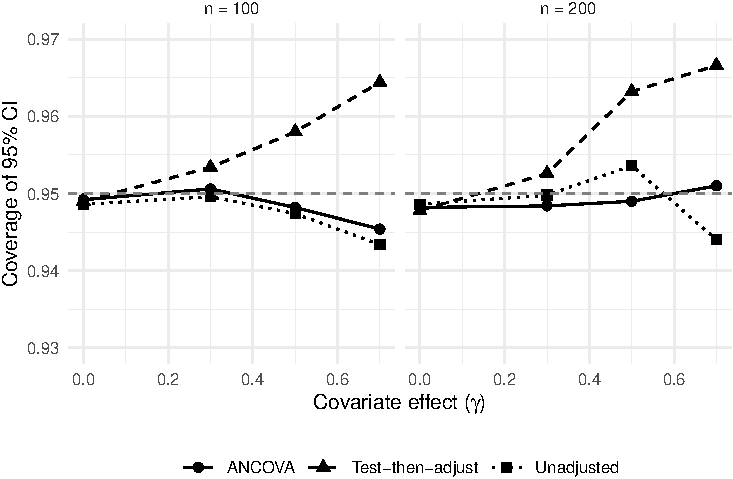
\includegraphics[keepaspectratio,alt={Empirical coverage of 95\% confidence intervals across analysis strategies. The horizontal dashed line marks nominal 95\% coverage.}]{report_files/figure-latex/coverage-plot-1.pdf}}
\caption{Empirical coverage of 95\% confidence intervals across analysis
strategies. The horizontal dashed line marks nominal 95\% coverage.}
\end{figure}

Figure 2 demonstrates that all three strategies maintain approximately
nominal coverage. The test-then-adjust strategy shows minor coverage
perturbations in some scenarios, consistent with the theoretical
concerns about data-dependent model selection.

\section{Discussion}\label{discussion}

\subsection{Summary of Objective
Criteria}\label{summary-of-objective-criteria}

Based on the theoretical literature, empirical evidence, and regulatory
guidance, we propose the following objective criteria for covariate
adjustment in the primary analysis of an RCT.

\textbf{When to adjust:}

\begin{enumerate}
\def\labelenumi{\arabic{enumi}.}
\tightlist
\item
  \emph{Always}, if prognostic covariates are available and
  pre-specified. The decision to adjust should never be based on
  observed baseline balance
  (\citeproc{ref-sennTestingBaselineBalance1994a}{Senn 1994},
  \citeproc{ref-sennSevenMyths2013}{2013}).
\item
  \emph{Always} include stratification variables used in the
  randomization design as covariates in the analysis
  (\citeproc{ref-kahanImproper2012}{Kahan and Morris 2012};
  \citeproc{ref-emaBaselineCovariates2015}{European Medicines Agency
  2015}; \citeproc{ref-fdaCovariateAdjustment2023}{US Food and Drug
  Administration 2023}).
\item
  \emph{Always} include the baseline measurement of the outcome
  variable, if available (\citeproc{ref-vickersBaseline2001}{Vickers and
  Altman 2001}; \citeproc{ref-sennChangeBaseline2006}{Senn 2006};
  \citeproc{ref-yangEfficiency2001}{Yang and Tsiatis 2001}).
\end{enumerate}

\textbf{Which covariates to adjust for:}

\begin{enumerate}
\def\labelenumi{\arabic{enumi}.}
\setcounter{enumi}{3}
\tightlist
\item
  Select covariates based on prior knowledge of their prognostic value
  -- from previous trials, meta-analyses, or established clinical
  understanding (\citeproc{ref-raabHowSelectCovariates2000}{Raab et al.
  2000}; \citeproc{ref-beachCovariates1989}{Beach and Meier 1989}).
\item
  The number of covariates should be small relative to the sample size.
  Raab et al. (\citeproc{ref-raabHowSelectCovariates2000}{2000}) provide
  a formula relating the benefit of adjustment to the number of subjects
  per covariate.
\item
  Do not select covariates based on the trial data itself (neither on
  baseline imbalance nor on observed covariate-outcome associations).
  Data-driven selection produces biased inference
  (\citeproc{ref-raabHowSelectCovariates2000}{Raab et al. 2000};
  \citeproc{ref-assmannSubgroupAnalysis2000}{Assmann et al. 2000}).
\end{enumerate}

\textbf{How to adjust:}

\begin{enumerate}
\def\labelenumi{\arabic{enumi}.}
\setcounter{enumi}{6}
\tightlist
\item
  For continuous outcomes: use ANCOVA (linear regression of \(Y\) on
  \(Z\) and \(X\)). Standard (OLS) or robust standard errors are both
  acceptable for balanced designs (\citeproc{ref-linAgnostic2013}{Lin
  2013}; \citeproc{ref-fdaCovariateAdjustment2023}{US Food and Drug
  Administration 2023}).
\item
  For binary outcomes: fit a logistic regression model and compute the
  marginal effect (standardization / g-computation) to obtain a risk
  difference or relative risk (\citeproc{ref-mooreCovariate2009}{Moore
  and Laan 2009}; \citeproc{ref-vanLanckerCovariate2024}{Van Lancker et
  al. 2024}). Alternatively, use a linear probability model or modified
  Poisson regression with robust standard errors.
\item
  For time-to-event outcomes: use a covariate-adjusted log-rank test
  (\citeproc{ref-yeLogRank2024}{Ye et al. 2024}) or estimate the
  restricted mean survival time with covariate adjustment
  (\citeproc{ref-diazSurvival2019}{Dı́az et al. 2019};
  \citeproc{ref-luLogRank2008}{Lu and Tsiatis 2008}).
\item
  Use robust (sandwich) standard errors to guard against model
  misspecification (\citeproc{ref-rosenblumRegression2009}{Rosenblum and
  Laan 2009}; \citeproc{ref-tsiatisCovariate2008}{Tsiatis et al. 2008};
  \citeproc{ref-fdaCovariateAdjustment2023}{US Food and Drug
  Administration 2023}).
\item
  Pre-specify all covariates and the analysis method in the statistical
  analysis plan. The primary analysis should contain no interaction
  terms (\citeproc{ref-emaBaselineCovariates2015}{European Medicines
  Agency 2015}).
\end{enumerate}

\subsection{Consistency with Regulatory
Guidance}\label{consistency-with-regulatory-guidance}

These criteria are fully consistent with the EMA guideline
(\citeproc{ref-emaBaselineCovariates2015}{European Medicines Agency
2015}) and the FDA final guidance
(\citeproc{ref-fdaCovariateAdjustment2023}{US Food and Drug
Administration 2023}). Both agencies endorse pre-specified covariate
adjustment as a tool for improving precision and recommend against
data-driven covariate selection. The FDA guidance specifically
recommends standardization for nonlinear models and robust variance
estimation.

\subsection{Limitations}\label{limitations}

The simulation presented here is deliberately simple, restricted to a
continuous outcome with a single covariate and no missing data. Real
trials involve multiple covariates, various outcome types, missing data,
and complications such as noncompliance and intercurrent events. The
estimand framework of ICH E9(R1)
(\citeproc{ref-ichE9R1Estimands2019}{ICH E9(R1) Expert Working Group
2019}) introduces additional considerations about what exactly is being
estimated. Nevertheless, the core message is robust: pre-specified
covariate adjustment improves efficiency without sacrificing validity,
across all outcome types and regulatory frameworks.

The simulation uses OLS-based standard errors rather than the sandwich
estimator. For the balanced designs considered here, the two are
asymptotically equivalent (\citeproc{ref-linAgnostic2013}{Lin 2013}),
but in practice, the sandwich estimator is more robust to
heteroscedasticity and is recommended by the FDA.

\section{Future Research}\label{future-research}

Several directions for future investigation emerge from this review:

\begin{enumerate}
\def\labelenumi{\arabic{enumi}.}
\item
  \textbf{Machine learning for covariate adjustment.} The FDA guidance
  does not yet address the use of machine learning methods for
  constructing prognostic scores. Schuler et al.
  (\citeproc{ref-schulerPrognostic2022}{2022}) showed that a prognostic
  score trained on external data can achieve the efficiency bound, but
  the operating characteristics of cross-validated or penalized
  approaches in the trial data itself remain under study. Van Lancker et
  al. (\citeproc{ref-vanLanckerGroupSequential2025}{2025}) explored
  combining covariate adjustment with group sequential and
  information-adaptive designs.
\item
  \textbf{Missing covariate data.} When baseline covariates are missing,
  the analyst faces a tradeoff between the efficiency gains from
  adjustment and the potential bias from ad hoc handling of missingness.
  Multiple imputation and augmented estimators are active research
  areas.
\item
  \textbf{Cluster-randomized and crossover trials.} The theory reviewed
  here applies primarily to individually randomized, parallel-group
  trials. Extensions to cluster randomization and crossover designs
  present additional methodological challenges.
\item
  \textbf{Software tools.} The R package \texttt{estimatr} implements
  Lin's regression estimator via the \texttt{lm\_lin()} function.
  Broader software implementing the standardization approach for various
  outcome types would make best practices more accessible.
\item
  \textbf{Harmonization of conditional and marginal frameworks.} The
  tension between conditional effects (natural for clinicians reasoning
  about individual patients) and marginal effects (natural for
  regulators reasoning about populations) remains unresolved
  (\citeproc{ref-permuttCovariates2020}{Permutt 2020};
  \citeproc{ref-vanLanckerCovariate2024}{Van Lancker et al. 2024};
  \citeproc{ref-harrellCommentary2024}{Harrell 2024}).
\end{enumerate}

\section*{References}\label{references}
\addcontentsline{toc}{section}{References}

\protect\phantomsection\label{refs}
\begin{CSLReferences}{1}{1}
\bibitem[\citeproctext]{ref-altmanComparabilityRandomisedGroups1985}
Altman, Douglas G. 1985. {``Comparability of {Randomised Groups}.''}
\emph{Journal of the Royal Statistical Society Series D: The
Statistician} 34 (1): 125--36. \url{https://doi.org/10.2307/2987510}.

\bibitem[\citeproctext]{ref-assmannSubgroupAnalysis2000}
Assmann, Susan F., Stuart J. Pocock, Laura E. Enos, and Linda E. Kasten.
2000. {``Subgroup Analysis and Other (Mis)uses of Baseline Data in
Clinical Trials.''} \emph{Lancet} 355 (9209): 1064--69.
\url{https://doi.org/10.1016/S0140-6736(00)02039-0}.

\bibitem[\citeproctext]{ref-beachCovariates1989}
Beach, Mary Lind, and Paul Meier. 1989. {``Choosing Covariates in the
Analysis of Clinical Trials.''} \emph{Controlled Clinical Trials} 10 (4
Suppl): 161S--175S. \url{https://doi.org/10.1016/0197-2456(89)90055-X}.

\bibitem[\citeproctext]{ref-benkeserCovid2021}
Benkeser, David, Iván Diaz, Alex Luedtke, Jodi Segal, Daniel
Scharfstein, and Michael Rosenblum. 2021. {``Improving Precision and
Power in Randomized Trials for {COVID-19} Treatments Using Covariate
Adjustment, for Binary, Ordinal, and Time-to-Event Outcomes.''}
\emph{Biometrics} 77 (4): 1467--81.
\url{https://doi.org/10.1111/biom.13377}.

\bibitem[\citeproctext]{ref-colantuoniPrognostic2015}
Colantuoni, Elizabeth, and Michael Rosenblum. 2015. {``Leveraging
Prognostic Baseline Variables to Gain Precision in Randomized Trials.''}
\emph{Statistics in Medicine} 34 (18): 2602--17.
\url{https://doi.org/10.1002/sim.6507}.

\bibitem[\citeproctext]{ref-diazSurvival2019}
Dı́az, Iván, Elizabeth Colantuoni, Daniel F. Hanley, and Michael
Rosenblum. 2019. {``Improved Precision in the Analysis of Randomized
Trials with Survival Outcomes, Without Assuming Proportional Hazards.''}
\emph{Lifetime Data Analysis} 25 (3): 439--68.
\url{https://doi.org/10.1007/s10985-018-9428-5}.

\bibitem[\citeproctext]{ref-emaBaselineCovariates2015}
European Medicines Agency. 2015. \emph{Guideline on Adjustment for
Baseline Covariates in Clinical Trials}. EMA/CHMP/295050/2013. European
Medicines Agency.

\bibitem[\citeproctext]{ref-freedmanRegression2008}
Freedman, David A. 2008. {``On Regression Adjustments to Randomized
Experiments.''} \emph{Annals of Applied Statistics} 2 (1): 176--96.
\url{https://doi.org/10.1214/07-AOAS143}.

\bibitem[\citeproctext]{ref-harrellCommentary2024}
Harrell, Jr., Frank E. 2024. {``Commentary on van {Lancker} Et Al.''}
\emph{Clinical Trials} 21 (4): 412--14.
\url{https://doi.org/10.1177/17407745241251609}.

\bibitem[\citeproctext]{ref-hauckCovariates1998}
Hauck, Walter W., Sharon Anderson, and Sue M. Marcus. 1998. {``Should We
Adjust for Covariates in Nonlinear Regression Analyses of Randomized
Trials?''} \emph{Controlled Clinical Trials} 19 (3): 249--56.
\url{https://doi.org/10.1016/S0197-2456(97)00147-5}.

\bibitem[\citeproctext]{ref-hernandezImpact2006}
{Hernandez, Adrian V., Ewout W. Steyerberg, Isabel Butcher, et al.}
2006. {``Adjustment for Strong Predictors of Outcome in Traumatic Brain
Injury Trials: 25\% Reduction in Sample Size Requirements in the
{IMPACT} Study.''} \emph{Journal of Neurotrauma} 23 (9): 1295--303.
\url{https://doi.org/10.1089/neu.2006.23.1295}.

\bibitem[\citeproctext]{ref-hernandezPower2004}
Hernandez, Adrian V., Ewout W. Steyerberg, and J. Dik F. Habbema. 2004.
{``Covariate Adjustment in Randomized Controlled Trials with Dichotomous
Outcomes Increases Statistical Power and Reduces Sample Size
Requirements.''} \emph{Journal of Clinical Epidemiology} 57 (5):
454--60. \url{https://doi.org/10.1016/j.jclinepi.2003.09.014}.

\bibitem[\citeproctext]{ref-ichE9R1Estimands2019}
ICH E9(R1) Expert Working Group. 2019. \emph{Addendum on Estimands and
Sensitivity Analysis in Clinical Trials to the Guideline on Statistical
Principles for Clinical Trials}. International Council for
Harmonisation.

\bibitem[\citeproctext]{ref-ichE9Statistical1999}
ICH Expert Working Group. 1999. {``{ICH} {E9}: Statistical Principles
for Clinical Trials.''} \emph{Statistics in Medicine} 18 (15): 1905--42.
\url{https://doi.org/10.1002/(SICI)1097-0258(19990815)18:15\%3C1905::AID-SIM188\%3E3.0.CO;2-F}.

\bibitem[\citeproctext]{ref-kahanImproper2012}
Kahan, Brennan C., and Tim P. Morris. 2012. {``Improper Analysis of
Trials Randomised Using Stratified Blocks or Minimisation.''}
\emph{Statistics in Medicine} 31 (4): 328--40.
\url{https://doi.org/10.1002/sim.4431}.

\bibitem[\citeproctext]{ref-lesaffreNonparametric2003}
Lesaffre, Emmanuel, and Stephen Senn. 2003. {``A Note on Non-Parametric
{ANCOVA} for Covariate Adjustment in Randomized Clinical Trials.''}
\emph{Statistics in Medicine} 22 (23): 3583--96.
\url{https://doi.org/10.1002/sim.1583}.

\bibitem[\citeproctext]{ref-linAgnostic2013}
Lin, Winston. 2013. {``Agnostic Notes on Regression Adjustments to
Experimental Data: Reexamining {Freedman}'s Critique.''} \emph{Annals of
Applied Statistics} 7 (1): 295--318.
\url{https://doi.org/10.1214/12-AOAS583}.

\bibitem[\citeproctext]{ref-luLogRank2008}
Lu, Xiaomin, and Anastasios A. Tsiatis. 2008. {``Improving the
Efficiency of the Log-Rank Test Using Auxiliary Covariates.''}
\emph{Biometrika} 95 (3): 679--94.
\url{https://doi.org/10.1093/biomet/asn003}.

\bibitem[\citeproctext]{ref-mooreCovariate2009}
Moore, Kelly L., and Mark J. van der Laan. 2009. {``Covariate Adjustment
in Randomized Trials with Binary Outcomes: Targeted Maximum Likelihood
Estimation.''} \emph{Statistics in Medicine} 28 (1): 39--64.
\url{https://doi.org/10.1002/sim.3445}.

\bibitem[\citeproctext]{ref-morrisPlanning2022}
Morris, Tim P., A. Sarah Walker, Elizabeth J. Williamson, and Ian R.
White. 2022. {``Planning a Method for Covariate Adjustment in
Individually Randomised Trials: A Practical Guide.''} \emph{Trials} 23
(1): 328. \url{https://doi.org/10.1186/s13063-022-06097-z}.

\bibitem[\citeproctext]{ref-permuttCovariates2020}
Permutt, Thomas. 2020. {``Do Covariates Change the Estimand?''}
\emph{Statistics in Biopharmaceutical Research} 12 (1): 45--53.
\url{https://doi.org/10.1080/19466315.2019.1647874}.

\bibitem[\citeproctext]{ref-pocockSubgroupAnalysisCovariate2002}
Pocock, Stuart J., Susan E. Assmann, Laura E. Enos, and Linda E. Kasten.
2002. {``Subgroup Analysis, Covariate Adjustment and Baseline
Comparisons in Clinical Trial Reporting: Current Practiceand
Problems.''} \emph{Statistics in Medicine} 21 (19): 2917--30.
\url{https://doi.org/10.1002/sim.1296}.

\bibitem[\citeproctext]{ref-raabHowSelectCovariates2000}
Raab, Gillian M, Simon Day, and Jill Sales. 2000. {``How to {Select
Covariates} to {Include} in the {Analysis} of a {Clinical Trial}.''}
\emph{Controlled Clinical Trials} 21 (4): 330--42.
\url{https://doi.org/10.1016/S0197-2456(00)00061-1}.

\bibitem[\citeproctext]{ref-robinsonCovariate1991}
Robinson, L. D., and N. P. Jewell. 1991. {``Some Surprising Results
about Covariate Adjustment in Logistic Regression Models.''}
\emph{International Statistical Review} 59 (2): 227--40.
\url{https://doi.org/10.2307/1403444}.

\bibitem[\citeproctext]{ref-rosenblumRegression2009}
Rosenblum, Michael, and Mark J. van der Laan. 2009. {``Using Regression
Models to Analyze Randomized Trials: Asymptotically Valid Hypothesis
Tests Despite Incorrectly Specified Models.''} \emph{Biometrics} 65 (3):
937--45. \url{https://doi.org/10.1111/j.1541-0420.2008.01177.x}.

\bibitem[\citeproctext]{ref-schulerPrognostic2022}
Schuler, Alejandro, David Walsh, Diana Hall, John Walsh, and Charles
Fisher. 2022. {``Increasing the Efficiency of Randomized Trial Estimates
via Linear Adjustment for a Prognostic Score.''} \emph{International
Journal of Epidemiology} 51 (4): 1150--58.
\url{https://doi.org/10.1093/ije/dyac049}.

\bibitem[\citeproctext]{ref-sennTestingBaselineBalance1994a}
Senn, Stephen. 1994. {``Testing for Baseline Balance in Clinical
Trials.''} \emph{Statistics in Medicine} 13 (17): 1715--26.
\url{https://doi.org/10.1002/sim.4780131703}.

\bibitem[\citeproctext]{ref-sennChangeBaseline2006}
Senn, Stephen. 2006. {``Change from Baseline and Analysis of Covariance
Revisited.''} \emph{Statistics in Medicine} 25 (24): 4334--44.
\url{https://doi.org/10.1002/sim.2682}.

\bibitem[\citeproctext]{ref-sennSevenMyths2013}
Senn, Stephen. 2013. {``Seven Myths of Randomisation in Clinical
Trials.''} \emph{Statistics in Medicine} 32 (9): 1439--50.
\url{https://doi.org/10.1002/sim.5713}.

\bibitem[\citeproctext]{ref-steyerbergHeterogeneity2004}
Steyerberg, Ewout W., and Marinus J. C. Eijkemans. 2004.
{``Heterogeneity Bias: The Difference Between Adjusted and Unadjusted
Effects.''} \emph{Medical Decision Making} 24 (2): 145--53.
\url{https://doi.org/10.1177/0272989X03262285}.

\bibitem[\citeproctext]{ref-tsiatisCovariate2008}
Tsiatis, Anastasios A., Marie Davidian, Min Zhang, and Xiaomin Lu. 2008.
{``Covariate Adjustment for Two-Sample Treatment Comparisons in
Randomized Clinical Trials: A Principled yet Flexible Approach.''}
\emph{Statistics in Medicine} 27 (23): 4658--77.
\url{https://doi.org/10.1002/sim.3113}.

\bibitem[\citeproctext]{ref-turnerCovariate2012}
{Turner, Elizabeth L., Pablo Perel, Tim Clayton, et al.} 2012.
{``Covariate Adjustment Increased Power in Randomized Controlled Trials:
An Example in Traumatic Brain Injury.''} \emph{Journal of Clinical
Epidemiology} 65 (5): 474--81.
\url{https://doi.org/10.1016/j.jclinepi.2011.08.012}.

\bibitem[\citeproctext]{ref-fdaCovariateAdjustment2023}
US Food and Drug Administration. 2023. \emph{Adjusting for Covariates in
Randomized Clinical Trials for Drugs and Biological Products: Guidance
for Industry}. US Food; Drug Administration.

\bibitem[\citeproctext]{ref-vanLanckerGroupSequential2025}
Van Lancker, Kelly, Joshua Betz, and Michael Rosenblum. 2025.
{``Combining Covariate Adjustment with Group Sequential,
Information-Adaptive Designs to Improve Randomized Trial Efficiency.''}
\emph{Biometrics} 81 (1): ujaf020.
\url{https://doi.org/10.1093/biom/ujaf020}.

\bibitem[\citeproctext]{ref-vanLanckerCovariate2024}
Van Lancker, Kelly, Frank Bretz, and Oliver Dukes. 2024. {``Covariate
Adjustment in Randomized Controlled Trials: General Concepts and
Practical Considerations.''} \emph{Clinical Trials} 21 (4): 399--411.
\url{https://doi.org/10.1177/17407745241251568}.

\bibitem[\citeproctext]{ref-vickersBaseline2001}
Vickers, Andrew J., and Douglas G. Altman. 2001. {``Statistics Notes:
Analysing Controlled Trials with Baseline and Follow up Measurements.''}
\emph{BMJ} 323 (7321): 1123--24.
\url{https://doi.org/10.1136/bmj.323.7321.1123}.

\bibitem[\citeproctext]{ref-yangEfficiency2001}
Yang, Lili, and Anastasios A. Tsiatis. 2001. {``Efficiency Study of
Estimators for a Treatment Effect in a Pretest-Posttest Trial.''}
\emph{American Statistician} 55 (4): 314--21.
\url{https://doi.org/10.1198/000313001753272466}.

\bibitem[\citeproctext]{ref-yeLogRank2024}
Ye, Ting, Jun Shao, and Yanyao Yi. 2024. {``Covariate-Adjusted Log-Rank
Test: Guaranteed Efficiency Gain and Universal Applicability.''}
\emph{Biometrika} 111 (2): 691--705.
\url{https://doi.org/10.1093/biomet/asad045}.

\bibitem[\citeproctext]{ref-yePractice2023}
Ye, Ting, Jun Shao, Yanyao Yi, and Qingyuan Zhao. 2023. {``Toward Better
Practice of Covariate Adjustment in Analyzing Randomized Clinical
Trials.''} \emph{Journal of the American Statistical Association} 118
(544): 2370--82. \url{https://doi.org/10.1080/01621459.2023.2179547}.

\bibitem[\citeproctext]{ref-zhangEfficiency2008}
Zhang, Min, Anastasios A. Tsiatis, and Marie Davidian. 2008.
{``Improving Efficiency of Inferences in Randomized Clinical Trials
Using Auxiliary Covariates.''} \emph{Biometrics} 64 (3): 707--15.
\url{https://doi.org/10.1111/j.1541-0420.2007.00976.x}.

\end{CSLReferences}

\end{document}
